\documentclass[11pt,a4paper]{article}

% ----------------------------------------------------------------------
% Pacchetti
% ----------------------------------------------------------------------
\usepackage[utf8]{inputenc}
\usepackage[T1]{fontenc}
\usepackage[italian]{babel}
\usepackage{amsmath,amssymb}
\usepackage{graphicx}
\usepackage{booktabs}
\usepackage{algorithm}
\usepackage{algpseudocode}
\usepackage{listings}
\usepackage{xcolor}
\usepackage{hyperref}
\usepackage{geometry}
\usepackage{caption}
\usepackage{subcaption}
\usepackage{float}

\geometry{margin=2.5cm}

\hypersetup{
    colorlinks=true,
    linkcolor=black,
    citecolor=black,
    urlcolor=blue
}

% ----------------------------------------------------------------------
% Stile per il codice OCaml
% ----------------------------------------------------------------------
\lstdefinelanguage{ocaml}{
    keywords={let, rec, in, match, with, function, fun, if, then, else, type, module, struct, sig, end, mutable, of, and, begin},
    keywordstyle=\color{blue}\bfseries,
    comment=[s]{(*}{*)},
    commentstyle=\color{gray}\itshape,
    stringstyle=\color{orange},
    morestring=[b]",
    sensitive=true,
    showstringspaces=false,
}
\lstset{
    language=ocaml,
    basicstyle=\ttfamily\small,
    breaklines=true,
    frame=single,
    tabsize=2,
    numbers=left,
    numberstyle=\tiny\color{gray},
}

% ----------------------------------------------------------------------
% Frontespizio
% ----------------------------------------------------------------------
\title{Risoluzione del Uncapacitated Facility Location Problem \\
       tramite metaeuristiche ILS e Simulated Annealing}
\author{Tommaso Bagiana, \\
        Corso di Computational Intelligence \\
       }
\date{\today}

\begin{document}

\maketitle

\begin{abstract}
Il presente lavoro affronta il problema della localizzazione di impianti (\emph{Facility
Location Problem}), nella sua variante non capacitata (UFLP), tramite
un approccio a due livelli: una metaeuristica esplora lo spazio delle configurazioni
binarie di apertura/chiusura degli impianti, mentre il sottoproblema di trasporto
associato a ciascuna configurazione viene risolto in modo esatto scegliendo la sede più vicina all'utente tra quelle aperte. Sono state
implementate e confrontate due metaeuristiche, \emph{Iterated Local Search} (ILS) e
\emph{Simulated Annealing} (SA), analizzandone i parametri, qualità delle
soluzioni e costo computazionale su istanze di dimensione crescente.
Il linguaggio scelto è stato OCaml per due caratteristiche principali. La prima è che il codice è particolarmente efficiente, la seconda è che OCaml è un linguaggio funzionale, il che permette di scrivere problemi matematici come la \emph{Facility Location} in modo naturale e flessibile.
\end{abstract}

\tableofcontents
\newpage

% ======================================================================
\section{Definizione del problema}
% ======================================================================

\subsection{Uncapacitated Facility Location Problem (UFLP)}

Dato un insieme di potenziali impianti $I = \{1, \dots, n\}$, ciascuno con costo di
apertura $f_i$, e un insieme di clienti $J = \{1, \dots, m\}$, ciascuno con domanda $d_j$ da
soddisfare, e detto $c_{ij}$ il costo di servire il cliente $j$ dall'impianto $i$, la
formulazione a programmazione lineare intera dell'UFLP è:

\begin{align}
    \min \quad & \sum_{i \in I} f_i x_i + \sum_{i \in I} \sum_{j \in J} c_{ij} d_j z_{ij} \\
    \text{s.t.} \quad & \sum_{i \in I} z_{ij} = 1 & \forall j \in J \label{eq:uflp-demand}\\
    & \sum_{j \in J} z_{ij} \le m x_i & \forall i \in I \label{eq:uflp-open}\\
    & x_i \in \{0,1\} & \forall i \in I \\
    & z_{ij} \in \{0,1\} & \forall i \in I, j \in J
\end{align}

dove $x_i$ indica se l'impianto $i$ è aperto e $z_{ij}$ è 1 se la facility $i$ fornisce il cliente $j$, 0 altrimenti.
Il vincolo~\eqref{eq:uflp-demand} impone che
ogni domanda sia interamente soddisfatta, mentre il vincolo~\eqref{eq:uflp-open}
impedisce di servire clienti da impianti chiusi.

% ======================================================================
\section{Dettagli implementativi}
% ======================================================================

\subsection{Struttura del progetto}

Il progetto è strutturato in un approccio ibrido: il motore algoritmico è implementato in OCaml. La scelta è ricaduta su questo linguaggio per massimizzare le prestazioni, inoltre ocaml è un linguaggio funzionale, caratteristica che lo rende flessibile adatto a problemi matematici. L'orchestrazione degli esperimenti e l'analisi dei risultati sono gestite tramite script Python. 

La directory principale del progetto espone la seguente gerarchia:
\begin{itemize}
    \item \textbf{\texttt{main\_program/}}: È un progetto gestito con Dune che contiene l'implementazione in OCaml del risolutore.
    \begin{itemize}
        \item \textbf{\texttt{lib/}}: Contiene i moduli della libreria. Troviamo \texttt{objective\_function.ml} per la valutazione delle soluzioni, \texttt{ils.ml} e \texttt{sa.ml} per l'esecuzione delle metaeuristiche, \texttt{reader.ml} per il parsing delle istanze da file testuali e \texttt{csv\_logger.ml} per tracciare e salvare i risultati.
        \item \textbf{\texttt{bin/main.ml}}: Contiene l'interfaccia a riga di comando (CLI) e funge da \emph{entry point} dell'eseguibile.
    \end{itemize}
    \item \textbf{Script Python (\texttt{tuning.py}, \texttt{analyze\_tuning.py}, \texttt{plot\_traces.py})}: Situati nella directory radice, questi file si occupano di avviare sistematicamente l'eseguibile OCaml passandogli i parametri, calcolare l'analisi di sensibilità sugli iperparametri e processare i tracciati di convergenza.
    \item \textbf{Directory grafiche e di output (\texttt{figs/}, \texttt{analysis\_output/})}: Raccolgono le visualizzazioni generate dagli script Python, impiegate all'interno di questa relazione per l'esposizione dei risultati.
\end{itemize}

\subsection{Interfaccia a riga di comando}

Il programma espone un'interfaccia a riga di comando che consente di selezionare l'istanza da risolvere, l'algoritmo (\verb|ils| o \verb|sa|) e i relativi iperparametri. Il flag \verb|-notrace| consente di disattivare il logging per-iterazione (utile per ridurre l'overhead durante le campagne di tuning su larga scala), mantenendo comunque attivo il logging aggregato su \verb|runs.csv|.

\subsection{Raccolta dati}

Ogni esecuzione produce una riga in \verb|runs.csv| con il costo della soluzione trovata, il tempo di esecuzione, l'iterazione in cui è stata trovata la soluzione migliore e la configurazione di parametri utilizzata. Quando il logging per-iterazione è attivo, viene inoltre prodotto un file \verb|trace.csv| per ciascuna esecuzione, contenente il costo della soluzione corrente e della migliore soluzione trovata ad ogni iterazione, utilizzato per le analisi di convergenza.

\subsection{Guida rapida alla compilazione e all'uso}
\label{sec:guida-uso}

\paragraph{Compilazione ed esecuzione del solver OCaml.}
Il progetto \texttt{main\_program/} è gestito con Dune. Per compilare:

\begin{verbatim}
cd main_program
dune build
\end{verbatim}

% TODO: verificare/completare i nomi esatti dei flag da riga di comando
% esposti da bin/main.ml (istanza, algoritmo, iperparametri, -notrace, ecc.)
% ed eventualmente sostituire l'esempio sotto con un caso reale.
Il programma può quindi essere eseguito tramite \texttt{dune exec}, specificando
l'istanza, l'algoritmo e i relativi iperparametri, ad esempio:

\begin{verbatim}
dune exec bin/main.exe -- -algo sa -instance <path_istanza> \
    -t0 100 -t_end 0.1 -alpha 0.9 -new_low 50 -seed 111
\end{verbatim}

Il flag \verb|-notrace| disattiva il logging per-iterazione (utile nelle
campagne di tuning su larga scala), mantenendo comunque attivo il logging
aggregato su \verb|runs.csv|.

\paragraph{Script Python.}
Gli esperimenti vengono orchestrati ed analizzati tramite tre script, eseguiti
nell'ordine seguente.

\begin{enumerate}
    \item \textbf{\texttt{tuning.py}}: lancia sistematicamente l'eseguibile
          OCaml sulla griglia di iperparametri (Tabella~\ref{tab:grid}),
          producendo \verb|runs.csv| e, se il logging non è disattivato, i
          file \verb|trace_*.csv|.
          % TODO: aggiungere qui l'esatta riga di comando di invocazione di
          % tuning.py (argomenti, eventuale file di configurazione), dato che
          % è uno script scritto autonomamente e non è descritto altrove in
          % questa relazione.

    \item \textbf{\texttt{analyze\_tuning.py}}: elabora \verb|runs.csv| e
          produce l'analisi di sensitivity (Sezioni~\ref{sec:risultati}):

\begin{verbatim}
python3 analyze_tuning.py runs.csv figs
\end{verbatim}

          Genera \verb|ils_sensitivity.png|, \verb|sa_sensitivity.png|, un
          grafico separato per ciascun parametro SA con effetto non
          trascurabile (es. \verb|sa_sensitivity_new_low.png|),
          \verb|quality_vs_time.png| e \verb|best_configs_summary.csv|. Lo
          script seleziona automaticamente, per ciascuna dimensione $n$, se
          include\-re i dati nelle medie aggregate in base alla completezza
          della copertura sperimentale (si veda la nota alla
          Sezione~\ref{sec:sa-sensitivity}); le esclusioni vengono
          stampate a schermo durante l'esecuzione.

    \item \textbf{\texttt{plot\_traces.py}}: elabora i file \verb|trace_*.csv|
          e produce le curve di convergenza (Figura~\ref{fig:convergence}):

\begin{verbatim}
python3 plot_traces.py --trace-dir ./traces --runs-csv runs.csv \
    --outdir figs_traces
\end{verbatim}

          Genera \verb|master_trace_long.csv| (tabella unica con tutte le
          traiettorie) e, per ogni $n$ trovato,
          \verb|convergence_n<N>.png| e \verb|convergence_n<N>_<algo>_variance.png|.
          Elabora i file uno alla volta e salva i risultati progressivamente,
          così un'interruzione a metà non fa perdere il lavoro già fatto:
          rilanciando lo stesso comando, i file già elaborati vengono saltati
          automaticamente. Altri flag utili: \verb|--no-resume| (riparte da
          zero), \verb|--no-collapse| (disattiva la compressione delle righe
          a costo invariato) e \verb|--skip-plots| (elabora solo i dati,
          utile con moltissimi file di trace, rimandando la generazione dei
          grafici a una chiamata successiva).
\end{enumerate}


% ======================================================================
\section{Approccio risolutivo}
\label{sec:approccio}
% ======================================================================
\subsection{Implementazione della Funzione Obiettivo}

Per valutare il costo totale di una determinata configurazione binaria $x$ di apertura degli impianti, è stata implementata una funzione obiettivo che calcola la somma dei costi fissi di apertura e dei costi di trasporto ottimi (associati al rispettivo sottoproblema). 

Di seguito viene riportato l'estratto del codice OCaml che si occupa di strutturare questa valutazione per il caso non capacitato (UFLP), isolando la matrice dei costi validi rispetto agli impianti attivi ed effettuando il calcolo posizionale del costo minimo per ciascun cliente:

\begin{lstlisting}[caption={Calcolo della funzione obiettivo per l'UFLP in OCaml.}, label={lst:objective_function}]
(* prende istanza e restituisce funzione obiettivo corrispondente *)
let objective_function instance x =
  match instance.u with
  | None ->
      let correct_cost_mat =
        Array.map2
          (fun cost_row is_open ->
             if is_open then cost_row
             else Array.make (Array.length cost_row) max_int)
          instance.c x
      in
      let rec aux j acc =
        if j < instance.m then
          let costo_spedizione =
            Array.fold_left (fun best row -> min best row.(j)) max_int correct_cost_mat
          in
          if costo_spedizione = max_int then
            Infeasible
          else
            aux (j + 1) (costo_spedizione * instance.d.(j) + acc)
        else
          Finite acc
      in
      aux 0 (opening_cost x instance.f) (* sommo costo spedizioni al costo di apertura *)
  | Some u -> raise Capacities
\end{lstlisting}

Nel frammento di codice sopra riportato (Listato~\ref{lst:objective_function}), si nota l'uso del tipo algebrico per gestire l'ammissibilità della soluzione (\texttt{Finite} o \texttt{Infeasible}) e il pattern matching per intercettare l'eventuale presenza di capacità (\texttt{Some u}).



% ======================================================================
\section{Metaeuristiche}
% ======================================================================

\subsection{Iterated Local Search (ILS)}

L'ILS implementato opera sul vettore binario $x$ di apertura/chiusura degli impianti, alternando fasi di ricerca locale e fasi di perturbazione:

\begin{itemize}
    \item \textbf{Perturbazione}: applicata tramite \emph{bit-flip} probabilistico su ciascuna componente di $x$, con probabilità di mutazione \verb|p_mut| configurabile.
    \item \textbf{Criterio di arresto}: numero massimo di iterazioni \verb|max_iterations|.
\end{itemize}

\begin{lstlisting}[caption={Local search e iterated search in OCaml.}, label={lst:iterated_search}]
(* TODO: l'operatore << qui sotto non e' standard OCaml (il confronto e' <).
   Se e' un operatore custom definito altrove per confrontare valori di tipo
   Finite/Infeasible, aggiungere una riga di testo che lo spieghi (altrimenti
   il listato sembra non compilare); se e' un refuso di trascrizione,
   sostituirlo con la funzione di confronto realmente usata in ils.ml. *)
let best_neighbor (x0, f_x0) f = (* f: objective function *)
  let neighbors    = neighbors_of x0 in
  let f_neighbors  = List.map f neighbors in
  let f_graph      = List.combine neighbors f_neighbors in
  let rec aux best = function
    [] -> best
    | (x, fx) :: rest ->
        if fx << snd best then aux (x, fx) rest
        else aux best rest
  in aux (x0, f_x0) f_graph

let rec local_search (x0, f_x0) f = (* passo coppia invece che solo x0 per evitare ricalcoli *)
  let (best, f_best) = best_neighbor (x0, f_x0) f in
  if f_best << f_x0 then
    local_search (best, f_best) f
  else
    (x0, f_x0)

let iterated_search ~rng ~log ~iterations ~p_mut ~instance ~f =
  let x0 = Array.init instance.n (fun _ -> Random.State.bool rng) in
  let (x0, f_x0) = local_search (x0, f x0) f in
  let rec aux current f_current best_iter i =
    (match log with
     | Some file ->
         Csv_logger.trace_logger ~file ~iteration:i
           ~current_cost:f_current ~best_cost:f_current
     | None -> ());
    if i < iterations then
      let tmp = perturbation rng current p_mut in
      let (next, f_next) = local_search (tmp, f tmp) f in
      if f_next << f_current then
        aux next f_next (i + 1) (i + 1)
      else
        aux current f_current best_iter (i + 1)
    else
      (current, f_current, best_iter, iterations)
  in
  aux x0 f_x0 0 0
\end{lstlisting}

\subsection{Simulated Annealing (SA)}

Il SA implementato adotta uno schema di raffreddamento, controllato dai seguenti parametri:

\begin{itemize}
    \item $t_0$: temperatura iniziale;
    \item $t_{end}$: temperatura finale (criterio di arresto);
    \item $\alpha$: fattore di raffreddamento geometrico, $t_{k+1} = \alpha \cdot t_k$;
    \item \verb|new_low|: lunghezza della catena di Markov (numero di iterazioni eseguite a temperatura costante prima di raffreddare).
\end{itemize}

Ad ogni iterazione viene generata una soluzione vicina tramite bit-flip di una componente di $x$; la mossa viene accettata se migliorativa, oppure con probabilità $e^{-\Delta / t}$ se peggiorativa. La funzione restituisce la \emph{migliore} soluzione incontrata durante l'intera esecuzione, e non semplicemente lo stato finale della catena.

\begin{lstlisting}[caption={Codice principale del Simulated Annealing.}, label={lst:sa_code}]
(* TODO: come sopra, verificare "<<" (confronto) e "%%" qui sotto (in OCaml
   il modulo e' l'operatore/keyword "mod", non "%%") rispetto al codice
   realmente compilato in sa.ml: se sono operatori custom vanno spiegati,
   altrimenti vanno corretti nel listato. *)
let accept_solution rng t f_old f_new = (* restituisce true se sceglie nuova soluzione *)
  match f_new, f_old with
  | Infeasible, _ ->
      false (* non accettiamo mai una mossa che porta a una soluzione infeasible *)
  | Finite _, Infeasible ->
      true (* qualunque soluzione feasible e' sempre meglio di una infeasible *)
  | Finite new_c, Finite old_c ->
      let delta = new_c - old_c in
      if delta <= 0 then true
      else
        let p = exp (-. (float_of_int delta) /. t) in
        (Random.State.float rng 1.0) < p


let simulated_annealing ~log ~rng ~t0 ~t_end ~alpha ~new_low ~instance ~f =
  let s0 = Array.init instance.n (fun _ -> Random.State.bool rng) in
  let f_s0 = f s0 in
  let rec aux i (s, f_s) (best, f_best) best_iter t =
    (match log with
     | Some file ->
         Csv_logger.trace_logger ~file ~iteration:i
           ~current_cost:f_s ~best_cost:f_best
     | None -> ());
    if t < t_end then
      (best, f_best, best_iter, i - 1)
    else
      let next = random_neighbor rng s instance.n in
      let f_next = f next in
      let accepted = accept_solution rng t f_s f_next in
      let best, f_best, best_iter =
        if f_next << f_best then (next, f_next, i) else (best, f_best, best_iter)
      in
      let t = if i %% new_low = 0 then alpha *. t else t in
      if accepted then
        aux (i + 1) (next, f_next) (best, f_best) best_iter t
      else
        aux (i + 1) (s, f_s) (best, f_best) best_iter t
  in
  aux 1 (s0, f_s0) (s0, f_s0) 0 t0
\end{lstlisting}

% ======================================================================
\section{Setup sperimentale}
% ======================================================================

Gli esperimenti sono stati condotti su istanze di dimensione crescente ($n \in \{5, 10, 20, 50, 100\}$, con $m = 2n$), ciascuna risolta con tre seed distinti (111, 222, 333).

Per ciascun algoritmo è stata condotta una campagna di tuning sui seguenti iperparametri:

\begin{table}[H]
\centering
\begin{tabular}{@{}ll@{}}
\toprule
\textbf{Algoritmo} & \textbf{Parametri esplorati} \\
\midrule
ILS & \verb|max_iterations| $\in \{10, 100, 1000, 10000\}$ \\
    & \verb|p_mut| $\in \{0.01, 0.05, 0.1\}$ \\
\midrule
SA  & $t_0 \in \{10, 50, 100, 300, 600\}$ \\
    & $\alpha \in \{0.85, 0.90, 0.95, 0.99\}$ \\
    & \verb|new_low| $\in \{10, 50, 100\}$ \\
\bottomrule
\end{tabular}
\caption{Griglia di iperparametri esplorata nella fase di tuning.}
\label{tab:grid}
\end{table}

% ======================================================================
\section{Risultati e analisi}
\label{sec:risultati}
% ======================================================================

\subsection{Taratura dei parametri di Iterated Local Search}

Per individuare una configurazione efficace dell'algoritmo ILS è stata effettuata un'analisi di sensibilità sui principali parametri, variando il numero massimo di iterazioni (\texttt{max\_iterations}) e la probabilità di perturbazione (\texttt{p\_mut}).

La Figura~\ref{fig:ils_tuning} riporta, rispettivamente, la frazione di esecuzioni che raggiungono la migliore soluzione osservata e il tempo medio di esecuzione al variare dei parametri.

\begin{figure}[H]
    \centering
    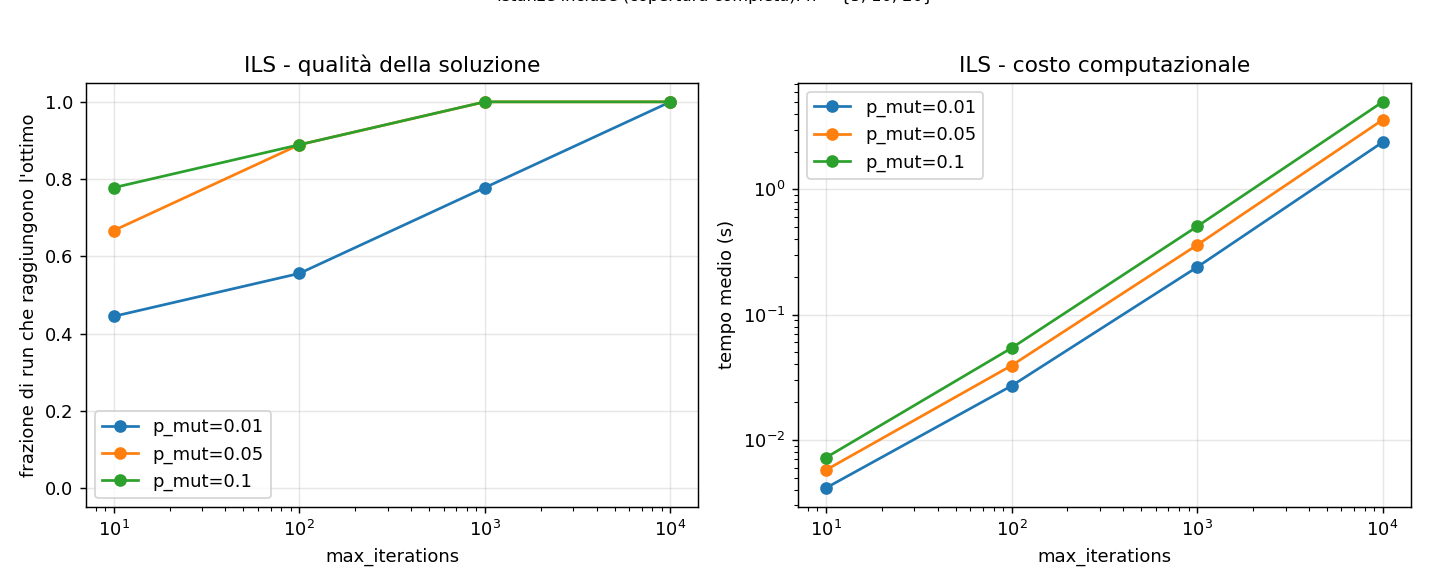
\includegraphics[width=\linewidth]{images/ils_sensitivity.png}
    \caption{Analisi di sensibilità dei parametri di Iterated Local Search. A sinistra è riportata la qualità della soluzione, espressa come frazione di esecuzioni che raggiungono la migliore soluzione osservata; a destra il tempo medio di esecuzione.}
    \label{fig:ils_tuning}
\end{figure}

Dal grafico relativo alla qualità della soluzione emerge che l'aumento del numero massimo di iterazioni migliora progressivamente le prestazioni dell'algoritmo. Tuttavia, oltre circa 1000 iterazioni il beneficio diventa trascurabile, poiché tutte le configurazioni raggiungono la migliore soluzione nella quasi totalità delle esecuzioni.

L'influenza della probabilità di perturbazione risulta invece più evidente per un numero ridotto di iterazioni. Il valore \texttt{p\_mut = 0.01} mostra una capacità di esplorazione inferiore, raggiungendo con minore frequenza la soluzione migliore. Al contrario, i valori \texttt{p\_mut = 0.05} e \texttt{p\_mut = 0.1} permettono di ottenere prestazioni significativamente migliori già con poche centinaia di iterazioni.

Il secondo grafico evidenzia il costo computazionale associato alle diverse configurazioni. Come prevedibile, il tempo di esecuzione aumenta all'aumentare del numero massimo di iterazioni. Inoltre, il valore \texttt{p\_mut = 0.01} richiede tempi sensibilmente maggiori per raggiungere prestazioni confrontabili con le altre configurazioni, mentre \texttt{p\_mut = 0.05} e \texttt{p\_mut = 0.1} mantengono un costo computazionale inferiore.

Considerando congiuntamente qualità della soluzione e tempo di esecuzione, la configurazione con \texttt{p\_mut = 0.05} e \texttt{max\_iterations = 100} rappresenta il miglior compromesso tra efficacia ed efficienza. Tale configurazione è stata pertanto adottata nelle successive prove di confronto e nell'analisi di scalabilità.


\subsection{Taratura dei parametri di Simulated Annealing}
\label{sec:sa-sensitivity}

Per capire l'ordine di importanza dei parametri di SA ho fissato un parametro alla volta ed ho calcolato la media della \emph{hit-rate} (percentuale di run che ha raggiunto il costo migliore).

\begin{table}[H]
\centering
\begin{tabular}{@{}lc@{}}
\toprule
\textbf{Parametro} & \textbf{Ampiezza effetto su hit-rate} \\
\midrule
$t_0$        & 0.354 \\
$\alpha$     & 0.174 \\
\texttt{new\_low} & 0.112 \\
$t_{end}$    & 0.004 \\
\bottomrule
\end{tabular}
\caption{Ampiezza dell'effetto marginale di ciascun iperparametro SA sulla frazione di run che raggiungono il costo ottimo.}
\label{tab:sa-importance}
\end{table}

Il risultato più rilevante è che $t_0$ ha un impatto maggiore di $\alpha$, contro l'aspettativa iniziale che avrebbe suggerito di concentrare l'analisi sulla coppia $(\alpha, \text{\texttt{new\_low}})$ in quanto concettualmente più legata al comportamento dell'algoritmo (velocità di raffreddamento e ampiezza dell'esplorazione a ciascuna temperatura). E' possibile che ciò sia causato dal fatto che ci siano più opzioni per $t_0$ e meno per $\texttt{new\_low}$.

La Figura~\ref{fig:sa-sensitivity} mostra quindi l'interazione tra $t_0$ e $\alpha$, i due parametri con maggiore impatto.

\begin{figure}[H]
    \centering
    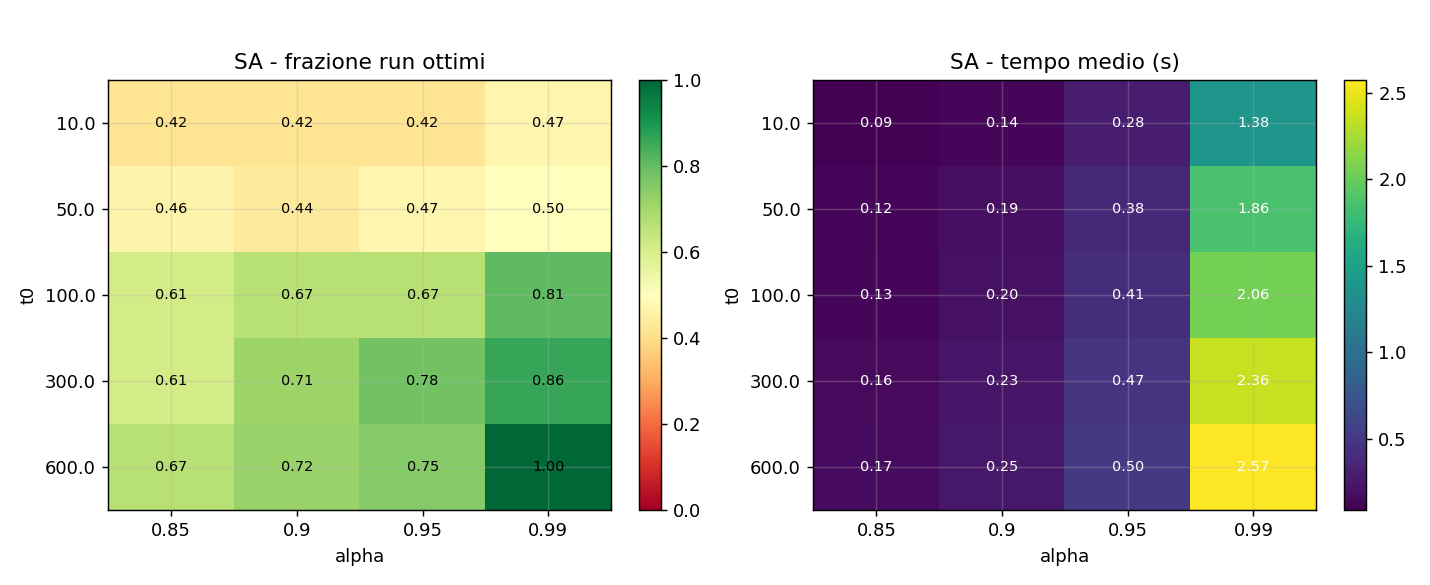
\includegraphics[width=\textwidth]{images/sa_sensitivity.png}
    \caption{SA — frazione di run che raggiungono l'ottimo e tempo medio, al variare di $t_0$ e $\alpha$ ($n \in \{5,10,20,50\}$).}
    \label{fig:sa-sensitivity}
\end{figure}

La hit-rate cresce in modo pressoché monotono lungo entrambi gli assi, dal minimo di 0.42 ($t_0=10$, $\alpha=0.85$) al massimo di 1.00 ($t_0=600$, $\alpha=0.99$): i due parametri hanno un effetto che si rinforza a vicenda. Il tempo medio cresce di pari passo, da 0.09s a 2.57s tra gli stessi due estremi, con un'eccezione: la colonna $\alpha=0.99$ è nettamente la più costosa in tempo (fino a 2.57s), più di quanto lo sia l'ultima riga $t_0=600$ (fino a 1.38s a $\alpha=0.85$). A parità di guadagno in hit-rate, alzare $t_0$ sembra più "efficiente" di alzare $\alpha$.

Il parametro restante non trascurabile, \verb|new_low|, viene mostrato separatamente in Figura~\ref{fig:sa-newlow}, marginalizzando su tutti gli altri parametri.

% PLACEHOLDER: inserire qui sa_sensitivity_new_low.png se esistente, o ignorare.
\begin{figure}[H]
    \centering
    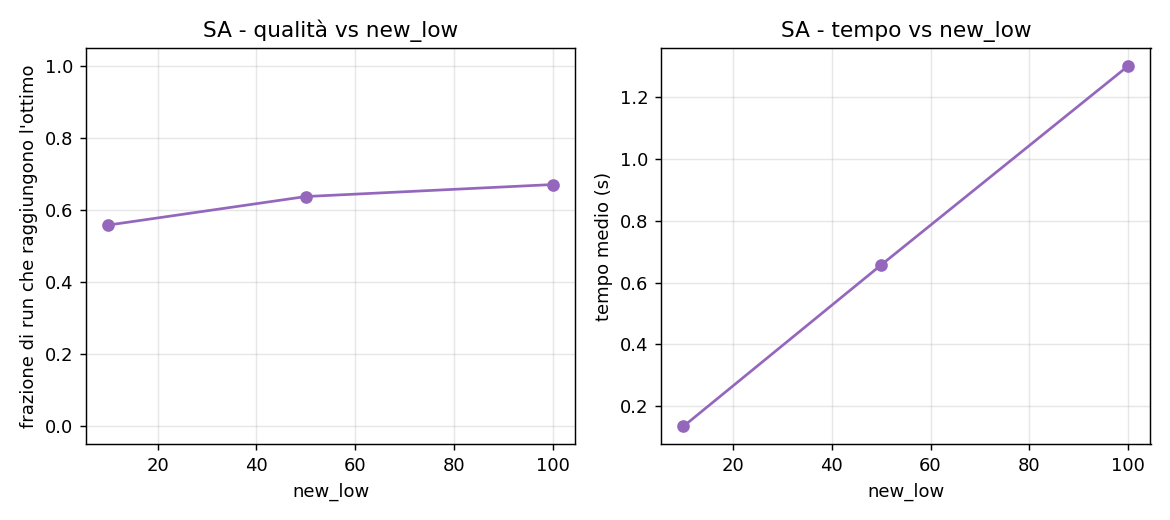
\includegraphics[width=0.7\textwidth]{images/sa_sensitivity_new_low.png}
    \caption{SA — frazione di run che raggiungono l'ottimo e tempo medio, al variare di \texttt{new\_low}.}
    \label{fig:sa-newlow}
\end{figure}

\subsection{Analisi delle curve di convergenza}

Per comprendere meglio il comportamento dinamico dei due algoritmi sono state analizzate le curve di convergenza del costo della migliore soluzione in funzione delle iterazioni. Per ciascuna dimensione del problema ($n=\{5,10,20,50\}$) sono stati eseguiti tre run indipendenti con seed differenti; nei grafici viene riportata la media delle traiettorie, mentre l'area ombreggiata rappresenta una deviazione standard.

Le Figure dalla~\ref{fig:conv_n5} alla~\ref{fig:conv_n100} mostrano il confronto tra Iterated Local Search (ILS) e Simulated Annealing (SA) al variare della dimensione dell'istanza.

\begin{figure}[H]
    \centering
    \begin{subfigure}{0.48\textwidth}
        \centering
        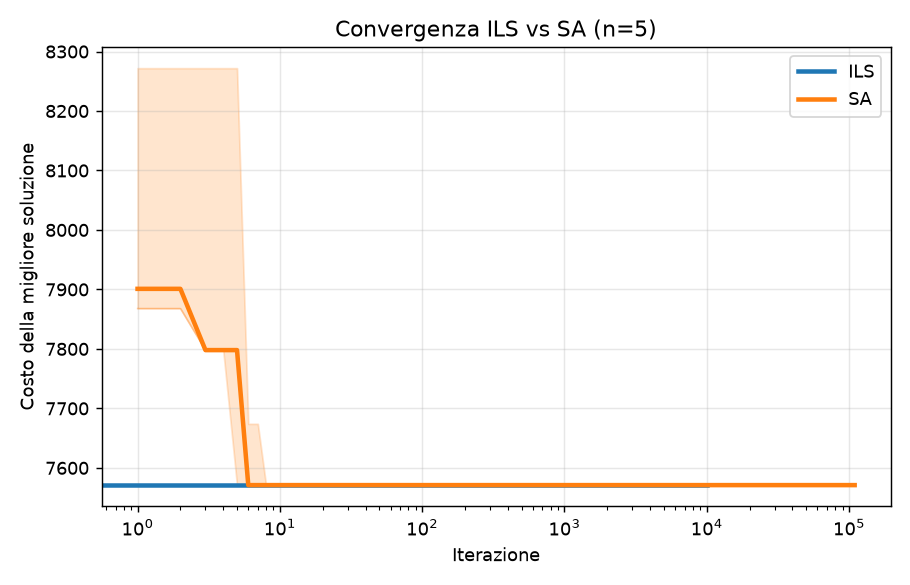
\includegraphics[width=\linewidth]{images/convergence_n5.png}
        \caption{$n=5$}
        \label{fig:conv_n5}
    \end{subfigure}
    \hfill
    \begin{subfigure}{0.48\textwidth}
        \centering
        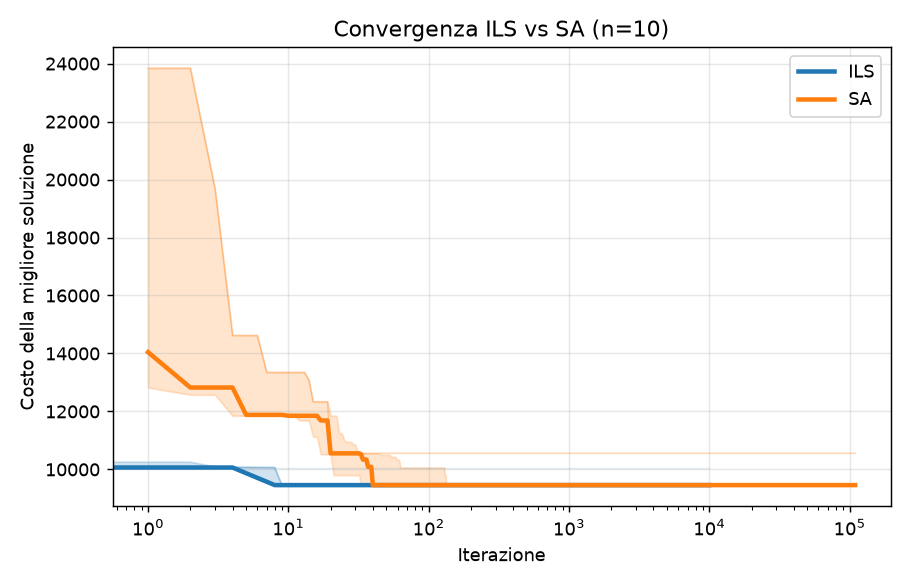
\includegraphics[width=\linewidth]{images/convergence_n10.png}
        \caption{$n=10$}
        \label{fig:conv_n10}
    \end{subfigure}

    \vspace{0.4cm}

    \begin{subfigure}{0.48\textwidth}
        \centering
        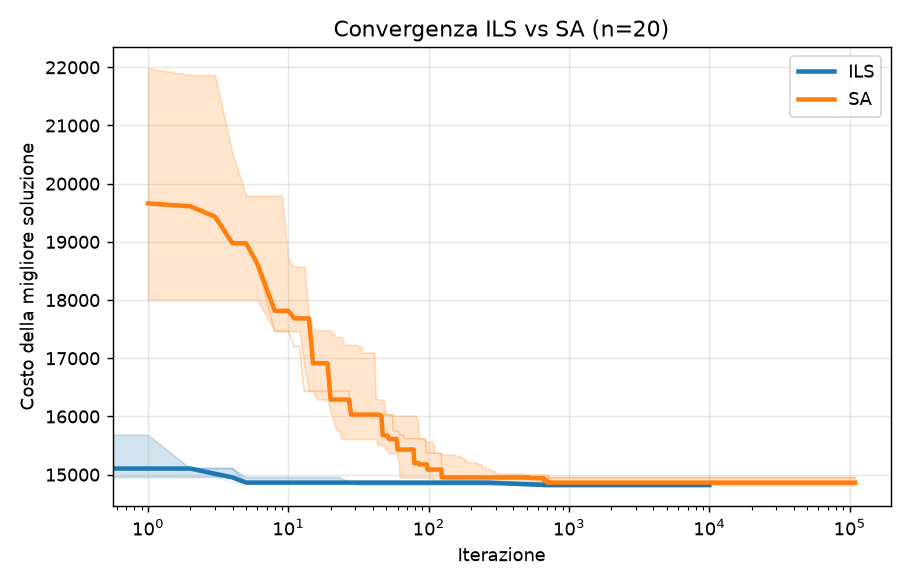
\includegraphics[width=\linewidth]{images/convergence_n20.png}
        \caption{$n=20$}
        \label{fig:conv_n20}
    \end{subfigure}
    \hfill
    \begin{subfigure}{0.48\textwidth}
        \centering
        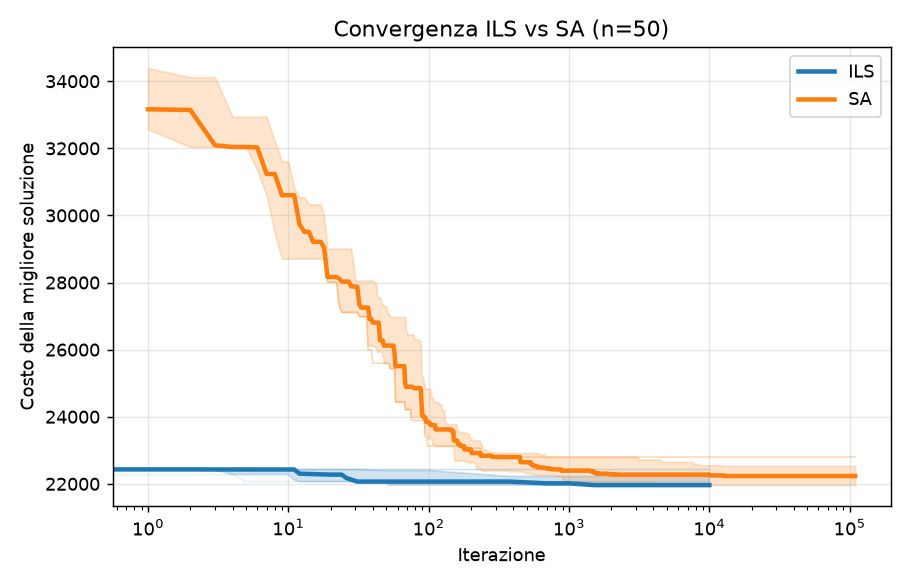
\includegraphics[width=\linewidth]{images/convergence_n50.png}
        \caption{$n=50$}
        \label{fig:conv_n50}
    \end{subfigure}

    \vspace{0.4cm}

    \begin{subfigure}{0.70\textwidth}
        \centering
        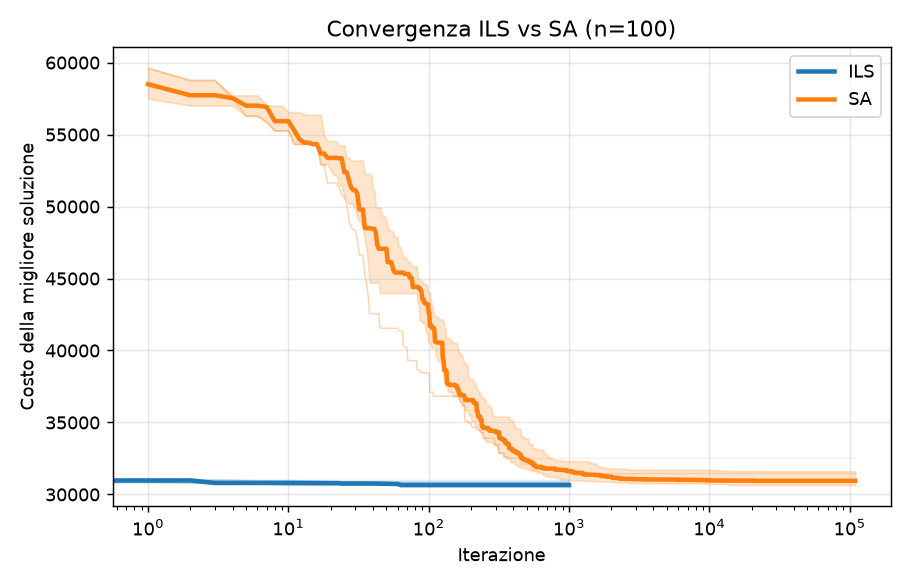
\includegraphics[width=\linewidth]{images/convergence_n100.png}
        \caption{$n=100$}
        \label{fig:conv_n100}
    \end{subfigure}

    \caption{Confronto delle curve di convergenza di ILS e SA per le diverse dimensioni del problema. Le linee rappresentano la media di tre esecuzioni indipendenti, mentre l'area ombreggiata indica $\pm1$ deviazione standard.}
    \label{fig:convergence}
\end{figure}

I risultati confermano le differenze già evidenziate dall'analisi quantitativa precedente.

L'Iterated Local Search mostra una convergenza estremamente rapida. In tutti gli esperimenti la migliore soluzione viene individuata nelle primissime iterazioni e successivamente il costo rimane pressoché costante. La banda di deviazione standard è inoltre molto ridotta, indicando che l'algoritmo produce risultati altamente riproducibili indipendentemente dal seed iniziale.

Al contrario, Simulated Annealing presenta un comportamento molto più graduale. Il costo diminuisce progressivamente durante il processo di raffreddamento, con miglioramenti distribuiti lungo un numero elevato di iterazioni. La maggiore ampiezza della banda di deviazione standard nelle prime fasi evidenzia una significativa variabilità tra le diverse esecuzioni, dovuta alla natura probabilistica dell'algoritmo. Tale variabilità tende però a ridursi man mano che la temperatura diminuisce e le diverse esecuzioni convergono verso soluzioni molto simili.

Per l'istanza più piccola ($n=5$) entrambi gli algoritmi raggiungono rapidamente la stessa soluzione finale. In questo caso SA necessita di poche iterazioni aggiuntive rispetto a ILS, ma la differenza risulta trascurabile.

Per $n=10$ emerge una differenza più evidente: ILS raggiunge quasi immediatamente un buon minimo locale, mentre SA continua a migliorare la soluzione fino a circa alcune decine di iterazioni, raggiungendo infine un costo leggermente inferiore. La maggiore dispersione iniziale delle traiettorie di SA indica una forte dipendenza dalle mosse casuali effettuate durante le prime fasi dell'esplorazione.

Anche per $n=20$ il comportamento osservato rimane sostanzialmente invariato. ILS converge quasi istantaneamente e mostra una variabilità minima tra i diversi seed. Simulated Annealing continua invece a migliorare la soluzione in modo graduale, riducendo progressivamente anche la variabilità tra le esecuzioni. Dopo circa un centinaio di iterazioni le traiettorie risultano quasi completamente sovrapposte.

Infine, per l'istanza più grande ($n=50$), la differenza tra i due algoritmi diventa ancora più marcata. ILS raggiunge rapidamente una soluzione stabile senza ulteriori miglioramenti significativi, mentre SA continua a esplorare lo spazio delle soluzioni per numerose iterazioni, ottenendo riduzioni del costo distribuite lungo tutto il processo di raffreddamento. Sebbene richieda un numero di iterazioni decisamente superiore, SA converge verso una soluzione finale sostanzialmente coincidente con quella ottenuta da ILS.

Nel complesso, queste curve confermano la diversa filosofia dei due metaeuristici. ILS privilegia uno sfruttamento intensivo dello spazio di ricerca, individuando rapidamente un buon minimo locale e mostrando un'elevata stabilità tra esecuzioni differenti. Simulated Annealing, invece, dedica una parte significativa dell'esecuzione all'esplorazione dello spazio delle soluzioni, accettando temporaneamente anche mosse peggiorative; ciò comporta una convergenza più lenta e una maggiore variabilità iniziale.

% ======================================================================
\section{Conclusioni}
% ======================================================================

Il presente lavoro ha affrontato la risoluzione dell'Uncapacitated Facility
Location Problem tramite due metaeuristiche, Iterated Local Search e
Simulated Annealing, costruite su una valutazione esatta della funzione
obiettivo (assegnazione di ciascun cliente alla sede aperta più economica) e
confrontate su istanze di dimensione crescente da $n=5$ a $n=100$.

\paragraph{Risultati principali.} Entrambi gli algoritmi si sono dimostrati
in grado di raggiungere il migliore costo noto sulla
quasi totalità delle istanze testate, purché configurati con un budget di
ricerca sufficiente. La differenza sostanziale non è tanto nella qualità
finale raggiungibile, quanto nel \emph{modo} in cui i due algoritmi vi
arrivano, come emerso dalle curve di convergenza (Sezione~\ref{sec:risultati}):
ILS individua una soluzione di ottima qualità entro poche decine di
iterazioni e vi resta sostanzialmente stabile, con una variabilità tra seed
minima; SA richiede invece alcuni ordini di grandezza di iterazioni in più,
mostrando un miglioramento progressivo e una variabilità iniziale
significativamente più ampia, che si riduce mano a mano che la temperatura
scende. Per le istanze più grandi ($n=50$, $n=100$) questa differenza si
accentua ulteriormente: SA impiega centinaia o migliaia di iterazioni per
avvicinarsi alla soluzione che ILS individua quasi immediatamente, pur
convergendo infine verso un costo finale comparabile.

\paragraph{Cosa conta per ciascun algoritmo.} L'analisi di sensitivity ha
mostrato che i due algoritmi non sono ugualmente sensibili a tutti i loro
iperparametri. Per ILS, sia \texttt{max\_iterations} che \texttt{p\_mut}
incidono sulla probabilità di raggiungere l'ottimo, ma con budget di
iterazioni ridotto (10--100) un \texttt{p\_mut} troppo basso (0.01) penalizza
sensibilmente la qualità rispetto a valori più esplorativi (0.05--0.1). Per
SA, la temperatura iniziale $t_0$ si è rivelata il parametro più
determinante (ampiezza dell'effetto marginale sulla hit-rate: 0.35, contro
0.17--0.22 di $\alpha$ e 0.11--0.15 di \texttt{new\_low}), mentre la
temperatura finale $t_{end}$ non ha mostrato alcun effetto misurabile nel
range testato (Tabella~\ref{tab:sa-importance}).

\paragraph{Limiti dello studio.} Vanno segnalati alcuni limiti nella
campagna sperimentale condotta. In primo luogo, il progetto copre
esclusivamente la variante non capacitata del problema (UFLP); l'estensione
al caso capacitato (CFLP) non è stata implementata.
In secondo luogo, la campagna di tuning di ILS non copre in modo completo la
combinazione di \texttt{max\_iterations} alto ($\geq 1000$) sulle istanze più
grandi ($n=50$, $n=100$): alcune run non sono state completate nei tempi a
disposizione, e i risultati relativi a quella porzione della griglia (esclusi
dalle medie riportate in Sezione~\ref{sec:risultati}) andrebbero considerati
preliminari. Infine, ciascuna configurazione è stata valutata su soli 3 seed:
sufficienti per individuare pattern generali netti, ma non per stime di
affidabilità statisticamente strette, specialmente per le configurazioni con
hit-rate intermedia (né vicina a 0 né a 1), dove la variabilità tra singole
esecuzioni pesa di più.


\end{document}